\documentclass[aspectratio=169]{beamer}
\usetheme{Madrid}
\usecolortheme{beaver}
\usepackage[utf8]{inputenc}
\usepackage[T1]{fontenc}
\usepackage{tikz}
\usepackage{amssymb}
\usepackage{graphicx}
\setbeamertemplate{navigation symbols}{}
\setbeamercolor{title}{fg=white,bg=cyan!60!black}
\setbeamercolor{frametitle}{fg=white,bg=cyan!50!black}
\setbeamercolor{block title}{bg=cyan!15,fg=black}
\setbeamercolor{block body}{bg=cyan!5,fg=black}

\title{G8 — Smart NPCs}
\subtitle{Lesson 2: Patrol Pattern}
\author{ByteForge --- Grade 7 --- Game Maker}
\date{}

\begin{document}

\begin{frame}
    \titlepage
\end{frame}

\begin{frame}{A direction variable that flips}
    \Large
    Storing "which way" as +1 or -1, flipped at a boundary, creates an endless back-and-forth patrol from one variable and two conditions.

    \begin{center}
    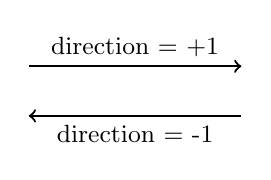
\begin{tikzpicture}[scale=0.9]

        \draw[->, thick] (0,0) -- (3,0);
        \draw[->, thick] (3,-0.7) -- (0,-0.7);
        \node[above] at (1.5,0) {\small direction = +1};
        \node[below] at (1.5,-0.7) {\small direction = -1};
    \end{tikzpicture}
    \end{center}
\end{frame}

\begin{frame}{Your Turn}
    \Large
    Open the student map, find \textbf{G8 — Smart NPCs}, and complete
    the \textbf{Patrol Pattern} challenge --- everything you just saw, they now do themselves.
\end{frame}

\end{document}
